\section{Interaction Rate}

\begin{frame}{Thermal bath}
\begin{columns}
    \begin{column}{0.5\textwidth}
    Interaction rate and Hubble constant:
        \begin{align}
	    \label{eq}
	    \begin{array}{ll}
		\Gamma > H \quad (coupled) \\
		\Gamma < H \quad (decoupled)\,,
	    \end{array}
        \end{align}
    \end{column}
    \begin{column}{0.5\textwidth}
\begin{center}
	\embedvideo*{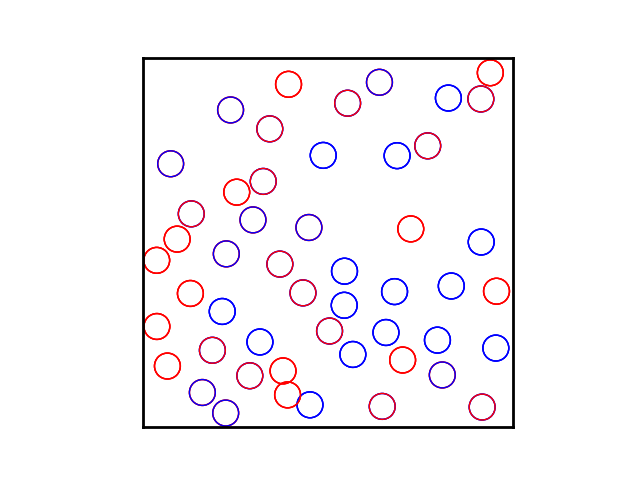
\includegraphics[width=\textwidth]{Figures/oie_transparent}}{collision.mp4}
\end{center}
    \end{column}
\end{columns}
\end{frame}
    
\begin{frame}
    \pause
\begin{block}{Interaction rate \cite{kolb}}
    \begin{equation}
	\Gamma=n\langle \sigma v \rangle =\frac{g}{16m^2\pi^2K_2(m/T)}\int_{4m^2}^\infty\sigma(s-4m^2)\sqrt{s}K_1\left(\frac{\sqrt{s}}{T}\right)ds\,.
    \end{equation}
\end{block}
\bigskip
\begin{itemize}
 \pause
 \item $|\overline{M}|^2_{1 + 2 \rightarrow 3 + 4}=|\overline{M}|^2_{3 + 4 \rightarrow 1 + 2}=|\overline{M}|^2$ \cite{kolb}
 \end{itemize}
\end{frame}
\begin{frame}{Amplitude}
Coupling terms ($\theta+\theta\rightarrow SM+\overline{SM}$): 
    \begin{align}
	\label{couplingterms}
	\begin{array}{ll}
	&\lambda_{\theta\theta h_i}=\dfrac{m_{h_1}^2}{v_\sigma}U_{2i}\,,\\	[8pt]
	&\lambda_{h_i SM SM}=U_{1i}g_{SM}\,.
	\end{array}
    \end{align}
    \pause
    Feynman diagram (s-channel):
    \begin{columns}
    \begin{column}{0.5\textwidth}
    \begin{center}
    \feynmandiagram[horizontal=a to b]{
    i1 [particle=\(\theta\)] --[scalar] a --[scalar] i2 [particle=\(\theta\)] ,
    a -- [boson,edge label=\(h_{1,2}\)] b, 
    f1 [particle=\(SM\)]  --[fermion] b -- [fermion]  f2[particle=\(\overline{SM}\)], 
    };
    \end{center}
    \end{column}
    \begin{column}{0.5\textwidth}
    \pause
    \begin{center}
    \begin{itemize}
        \item CalcHEP
    \end{itemize}
    \end{center}
    \end{column}
    \end{columns}
\end{frame}
\begin{frame}
    \begin{figure}
         \centering 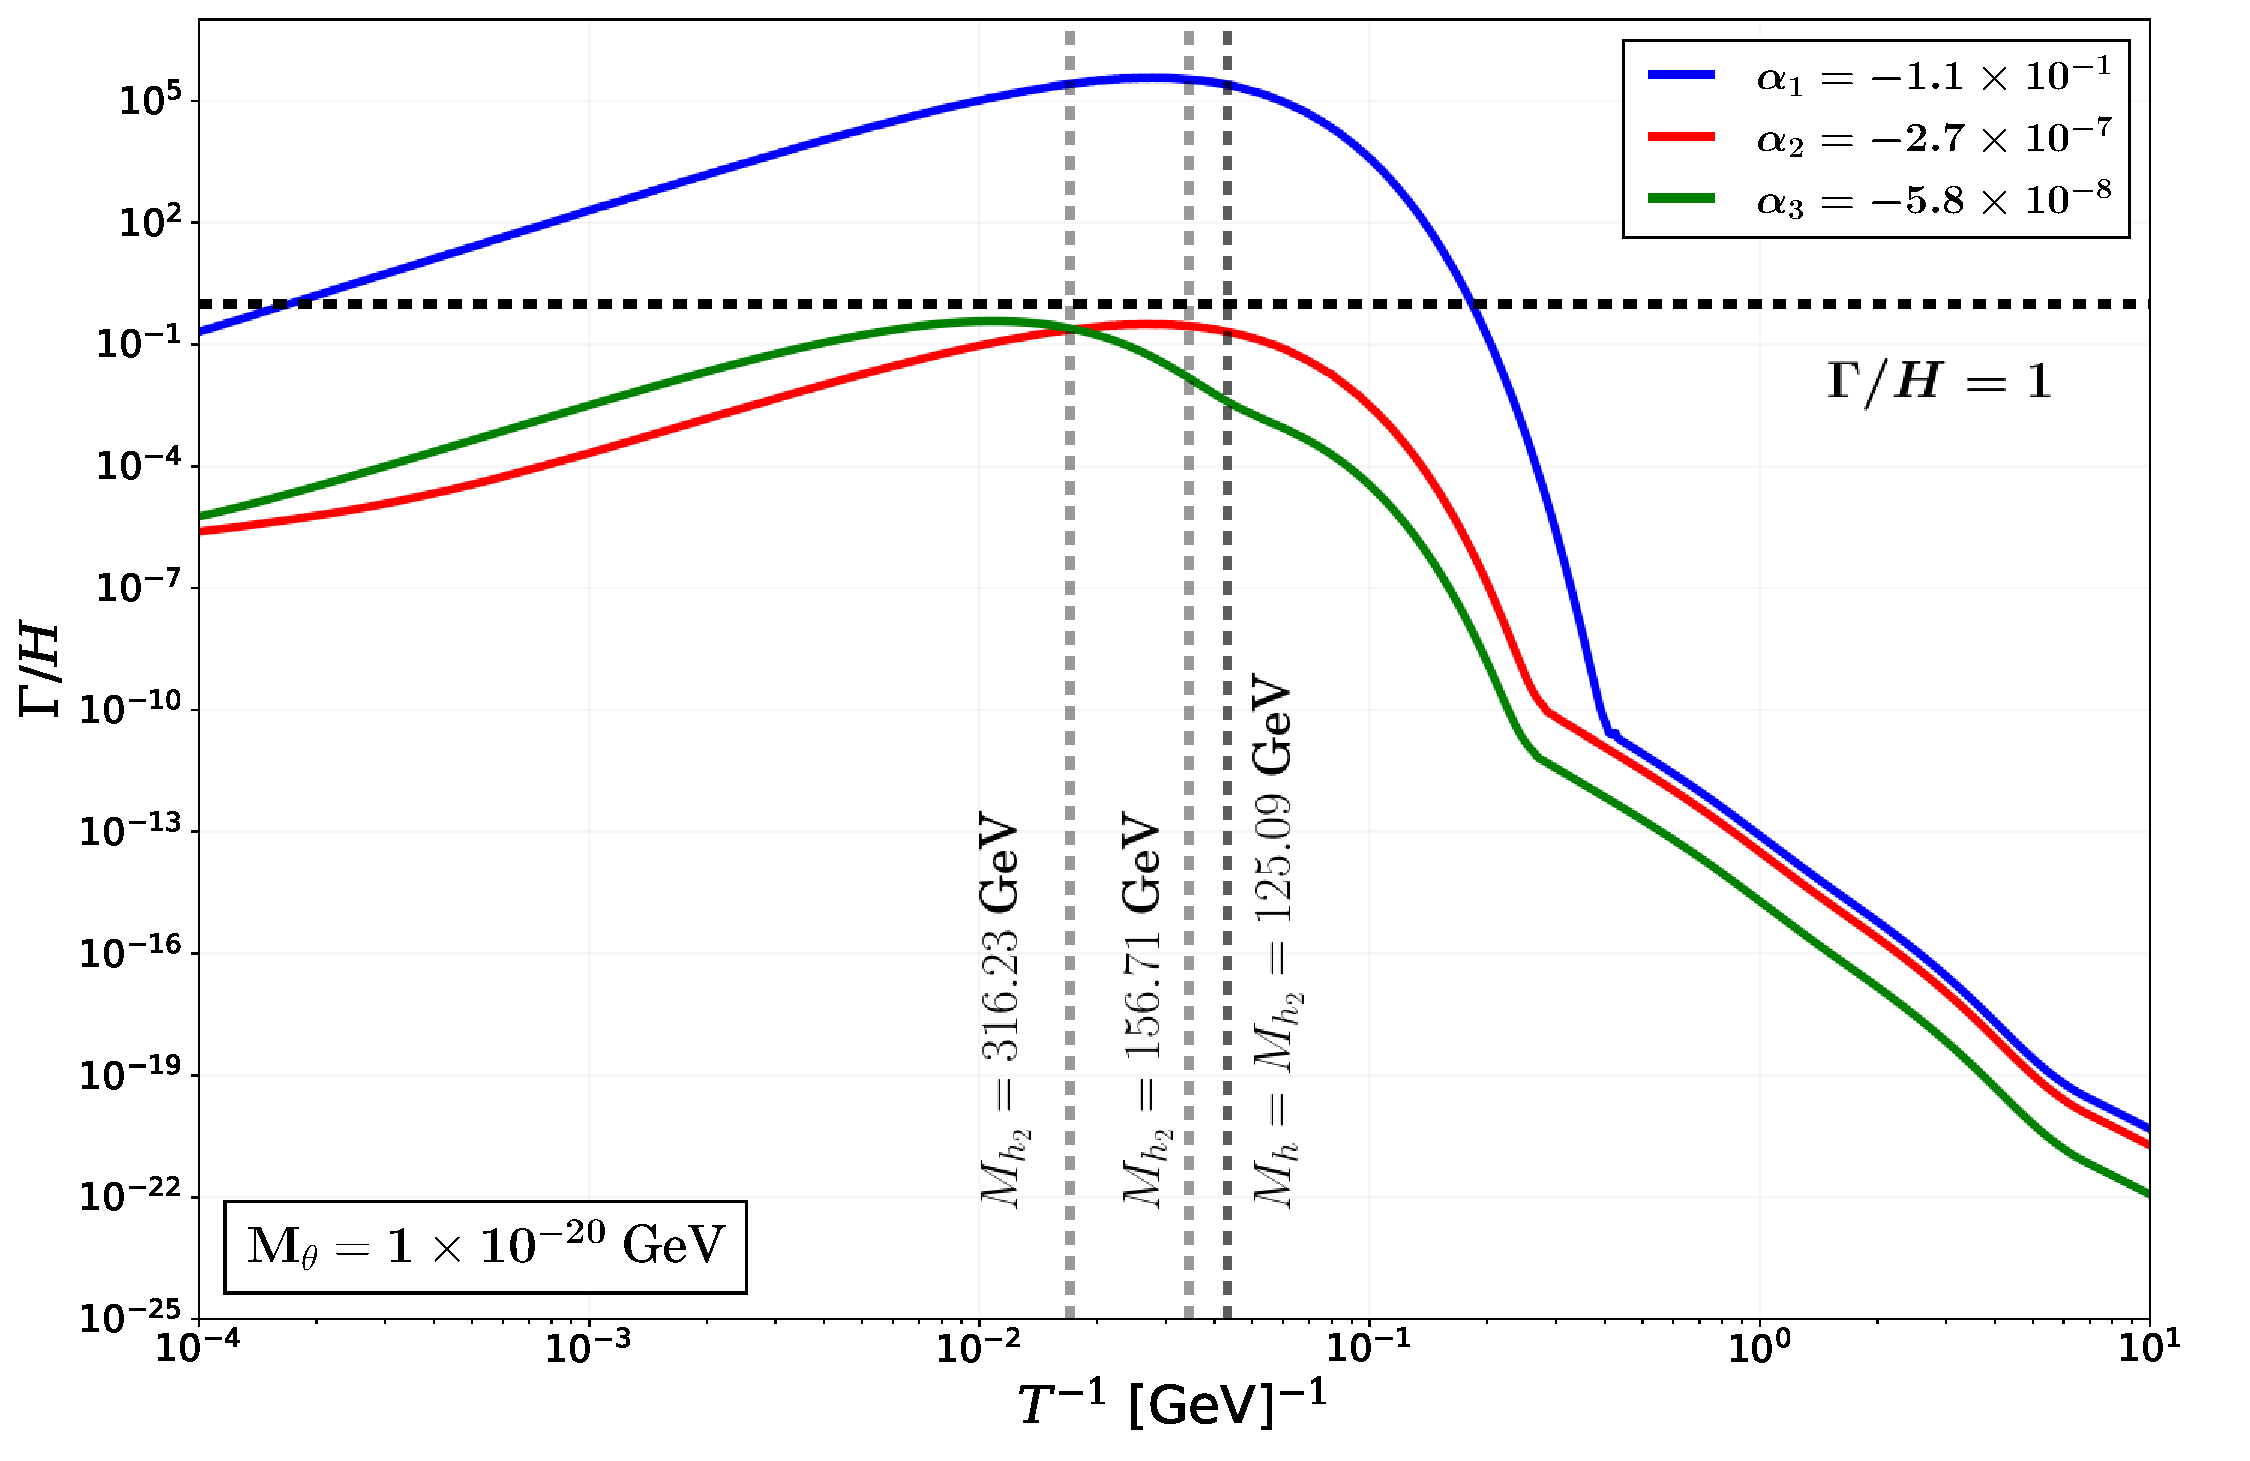
\includegraphics[width=.8\textwidth]{Figures/ratedm_equal.pdf}
        \caption{Rate of interaction divided by the Hubble constant assuming $m_h = m_{h_2}$ for $\lambda_H\sim0.26$, $\lambda_{H\phi}=2\times10^{-8}$ and $\lambda_\phi=0.1$}
        \label{fig:rot}
    \end{figure}
\end{frame}
\begin{frame}
        \begin{figure}
         \centering
         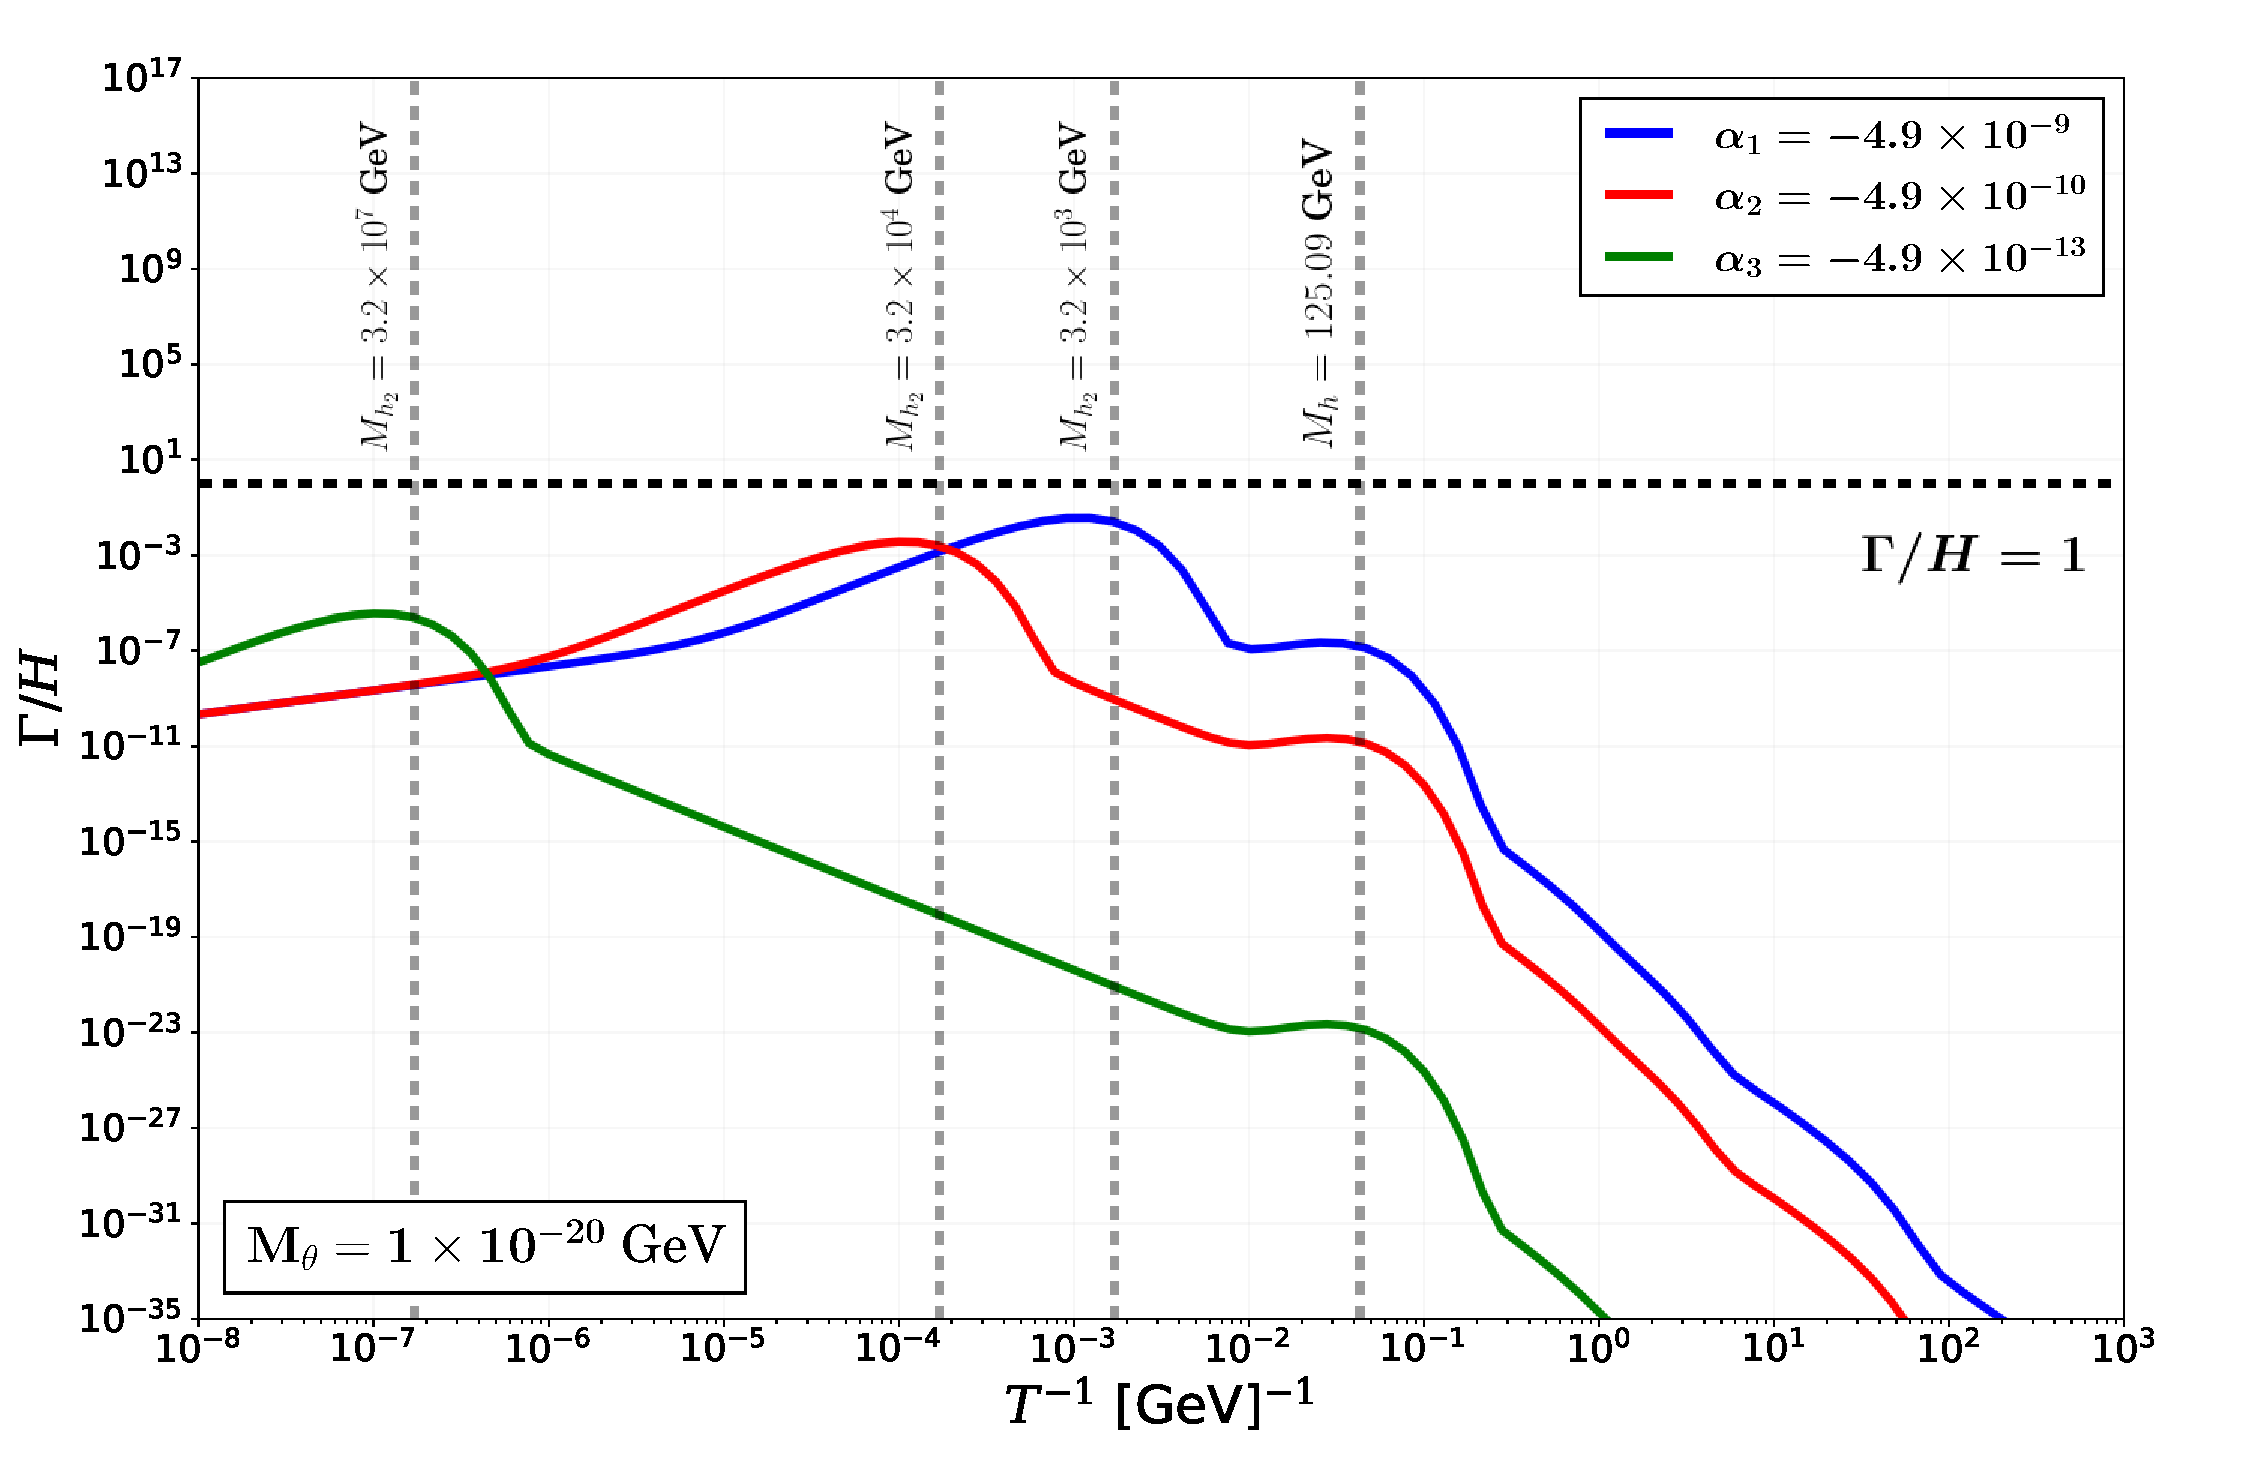
\includegraphics[width=.8\textwidth]{Figures/ratedm_greater.pdf}
        \caption{Rate of interaction divided by the Hubble constant assuming $m_h < m_{h_2}$ for $\lambda_H\sim0.26$, $\lambda_{H\phi}=2\times10^{-8}$ and $\lambda_\phi=0.1$}
        \label{fig:rot}
    \end{figure}
\end{frame}
\begin{frame}
        \begin{figure}
         \centering
         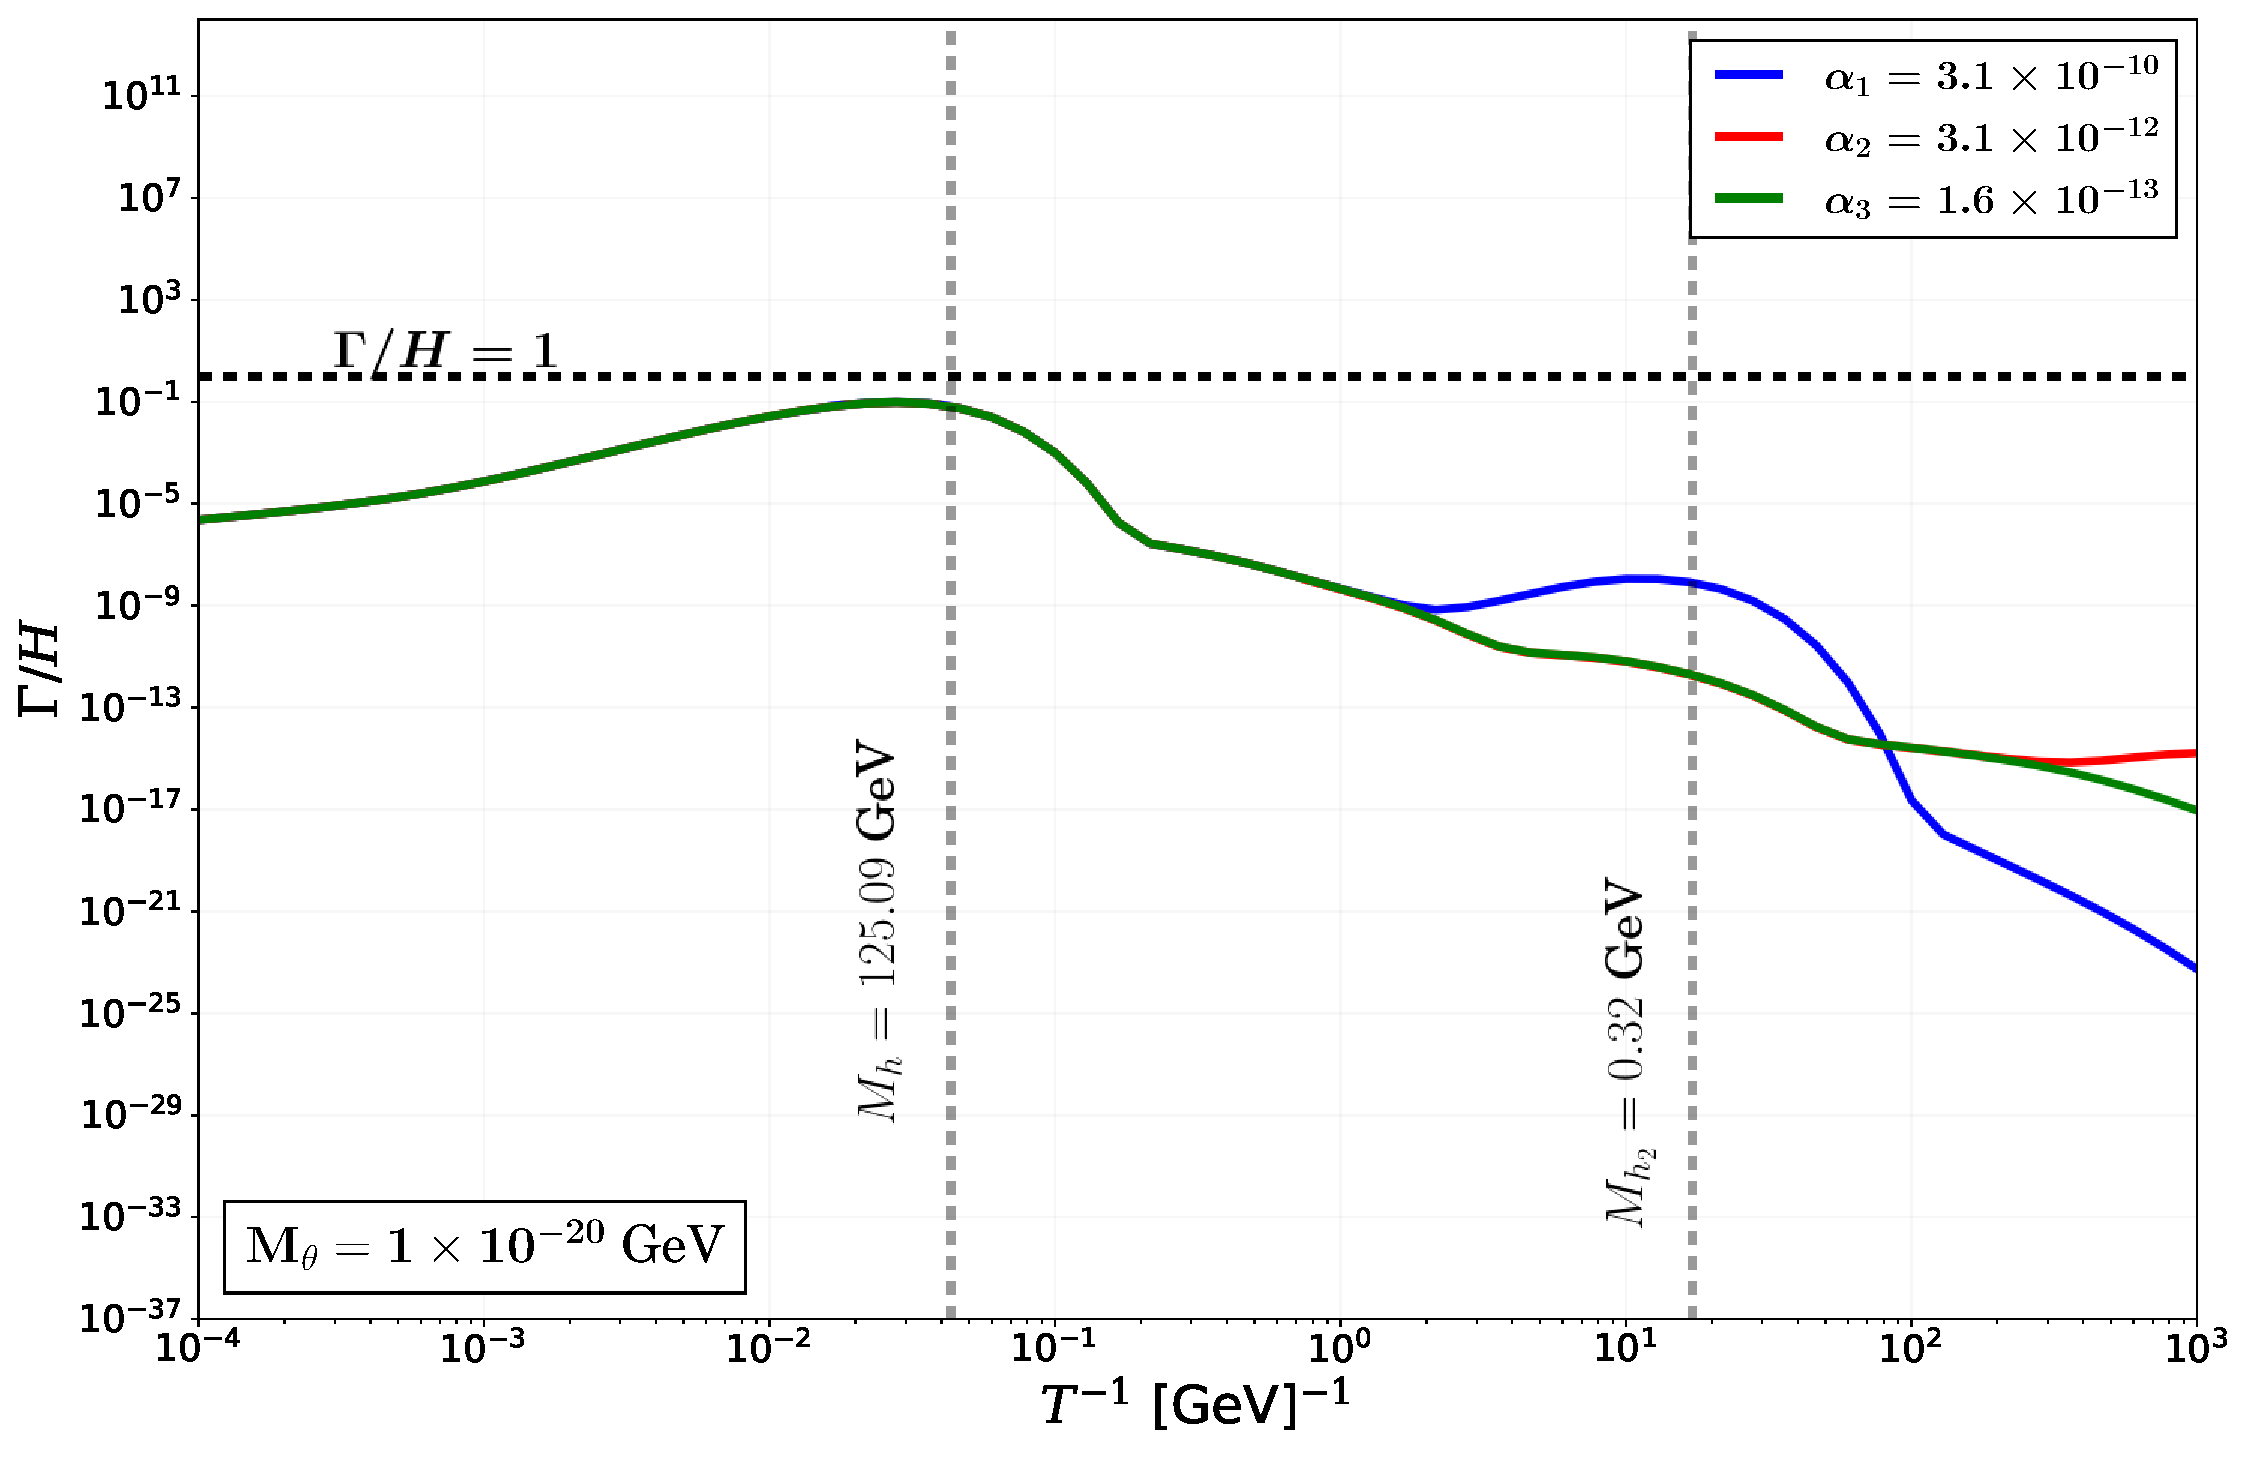
\includegraphics[width=.8\textwidth]{Figures/ratedm_lesser.pdf}
        \caption{Rate of interaction divided by the Hubble constant assuming $m_h > m_{h_2}$ for $\lambda_H\sim0.26$, $\lambda_{H\phi}=2\times10^{-8}$ and $\lambda_\phi=0.1$}
        \label{fig:rot}
    \end{figure}
\end{frame}